% HEADER %%%%%%%%%%%%%%%%%%%%%%%%%%%%%%%%%%%%%%%%%%%%%%%%%%%%%%%%%%%%%%%%%%%%%%%%%%%%%%%%%%%%%%%%%%%%%%%%%%%%%%%%%%%%%%%%%%%%%%%
\documentclass[a4paper,12pt]{article}

%New commands and Renew commands
\newcommand{\longtitle}[0]{Report} %For document title and cover
\newcommand{\shorttitle}[0]{Report} %For bookmark name, no special characters
\newcommand{\otoprule}{\midrule[\heavyrulewidth]} %bold rule with equal spacing up and down, ie bold midrule
\newcommand{\HRule}{\rule{\linewidth}{0.5mm}}
\newcommand{\ie}{\emph{i.e.}\xspace}
\newcommand{\Ie}{\emph{I.e.}\xspace}
\newcommand{\eg}{\emph{e.g.}\xspace}
\newcommand{\Eg}{\emph{E.g.}\xspace}

%Document language and encoding
\usepackage[english]{babel}
\usepackage[utf8]{inputenc}
\usepackage[T1]{fontenc}
\selectlanguage{english}

%Regular packages
%Regular packages in ALPHABETICAL order

\usepackage{amsmath}
\usepackage{amssymb}
\usepackage{array} 
\usepackage{booktabs}%to use \toprule and others
\usepackage{color}
\usepackage{colortbl}
\usepackage{ctable}%to use \toprule and others
\usepackage{epstopdf} % \def\pdfshellescape{1}
\usepackage{eurosym}
\usepackage{fixltx2e}
\usepackage{float}
\usepackage{framed}
\usepackage[bottom]{footmisc}%make sure footnotes stay at the bottom of the page
\usepackage{graphicx}
\usepackage{ifthen} %fancy references
\usepackage{indentfirst} %indent first paragraph after title
\usepackage{listingsutf8} \lstset{inputencoding=utf8/latin1} %acept accents (ie olá) in the listings environments
\usepackage{multicol}
\usepackage{siunitx} \sisetup{load-configurations=abbreviations} %use correctly typed SI units
\usepackage{subfig}
\usepackage{tabularx}%tables with variable space
\usepackage{thumbpdf} %thumbnails
\usepackage[dvipsnames]{xcolor} %must be loaded before tikz
\usepackage{tikz} %drawing
\usepackage[noindentafter]{titlesec}
\usepackage{url}
\usepackage{varioref} %fancy references
\usepackage{verbatim}
\usepackage{xspace}

\usepackage[plainpages=false,final]{hyperref} %should be the LAST package, unless specifically specified
\usepackage[all]{hypcap} %make sure links point to top of the captioned objects and not the captions themselves, must be called AFTER hyperreff
\usepackage[noabbrev]{cleveref} % the following loading order must be obeyed: variored, hyperref, cleveref (assuming all three are present) 


%Package Configurations sorted in ALPHABETICAL order

% \addtolength{\oddsidemargin}{-2.5cm} %change margins for odd numbered pages
% \addtolength{\evensidemargin}{-2.5cm} %change margins for even numbered pages
% \addtolength{\textwidth}{5cm} %change text width = margin de/increase in odd pages + margin de/increase in even pages
% \addtolength{\topmargin}{-2cm} %change margin on top
% \addtolength{\textheight}{4cm} %change text height (-2*\topmargin change)
\definecolor{castanho}{HTML}{ddd9c3}
\definecolor{preto}{rgb}{0,0,0}
\definecolor{shadecolor}{HTML}{cdc9c9} %for frames with gray background
\definecolor{rltblue}{rgb}{0,0,0.75}
\definecolor{rltgreen}{rgb}{0,0.5,0}
\definecolor{rltred}{rgb}{0.75,0,0}
\definecolor{tijolo}{cmyk}{0,0.64,0.65,0.61}
\epstopdfsetup{update,suffix=,verbose=false}
\graphicspath{
{figures/}
}
\hypersetup
{
        colorlinks=false,
        linkcolor=black,       % \ref{...} and \pageref{...}
        urlcolor=black,       % \href{...}{...} external (URL)
        filecolor=black,     % \href{...} local file
        pdftitle={\shorttitle},
        pdfauthor={Henrique Dantas, Luca Feltrin},
        pdfsubject={ET4171 Processor Design Project},
        pdfkeywords={VHDL, Leon3, Computer Arithmetic, Wallace Multiplier, Radix-4 Divider},
        pdfproducer={pdfLaTeX},
        bookmarksopen=true,
        pdfborder={0 0 0}
}
\numberwithin{equation}{section} %equation number include section
\numberwithin{figure}{section} %figure number include section
\numberwithin{table}{section} %table number include section
\titleformat{\part}[hang]{\bfseries\Large}{\thepart.}{0.5cm}{}
\titleformat{\section}[hang]{\bfseries\Large\color{NavyBlue}}{\thesection.}{0.2cm}{}
\titleformat{\subsection}[hang]{\bfseries\large\color{ProcessBlue}}{\thesubsection.}{0.2cm}{}
\titleformat{\subsubsection}[hang]{\normalfont\color{Emerald}}{\thesubsubsection.}{0.2cm}{}
% \titlespacing*{\part}{0cm}{-1.5cm}{1cm}
% \titlespacing*{\section}{0cm}{-1.5cm}{1cm}
% \titlespacing*{\subsection}{0.5cm}{1cm}{0.5cm}
% \titlespacing*{\subsubsection}{1cm}{1cm}{0.5cm}

% END OF HEADER %%%%%%%%%%%%%%%%%%%%%%%%%%%%%%%%%%%%%%%%%%%%%%%%%%%%%%%%%%%%%%%%%%%%%%%%%%%%%%%%%%%%%%%%%%%%%%%%%%%%%%%%%%%%%%%%

% COVER %%%%%%%%%%%%%%%%%%%%%%%%%%%%%%%%%%%%%%%%%%%%%%%%%%%%%%%%%%%%%%%%%%%%%%%%%%%%%%%%%%%%%%%%%%%%%%%%%%%%%%%%%%%%%%%%%%%%%%%%
\begin{document}

\pagenumbering{alph}
\begin{titlepage}
\begin{center}
\pdfbookmark[0]{\shorttitle}{Cover}

% Upper part of the page
\textsc{\LARGE TU Delft}\\[1cm]
\textsc{\Large ET4171 Processor Design Project}\\[1cm]

\includegraphics[scale=1.5]{tudelft-logo.jpg}

% Title
\HRule \\[0.4cm]
{\LARGE \bfseries Report}\\
\HRule \\[1cm]

% Author and supervisor
\begin{flushleft} \large
\emph{Authors:}\\ Henrique \textsc{Dantas} (4172922)\\Luca \textsc{Feltrin} (4270355) \\[1cm]
\end{flushleft}

%White space
\centering
\vspace{2cm}

% Bottom of the page
{\large \today}

\end{center}
\end{titlepage}

% END OF COVER %%%%%%%%%%%%%%%%%%%%%%%%%%%%%%%%%%%%%%%%%%%%%%%%%%%%%%%%%%%%%%%%%%%%%%%%%%%%%%%%%%%%%%%%%%%%%%%%%%%%%%%%%%%%%%%%%

% Table of Contents, List of figures and List of tables %%%%%%%%%%%%%%%%%%%%%%%%%%%%%%%%%%%%%%%%%%%%%%%%%%%%%%%%%%%%%%%%%%%%%%%%

%Table of Contents
\pdfbookmark[1]{Table of Contents}{index}
\pagenumbering{roman}
\phantomsection
\setcounter{page}{1}
\tableofcontents


%List of Figures
\newpage
\phantomsection
\addcontentsline{toc}{section}{List of Figures}
\listoffigures


%List of Tables
\phantomsection
% \vspace{5cm}
\addcontentsline{toc}{section}{List of Tables}
\listoftables


% END OF Table of Contents, List of figures and List of tables %%%%%%%%%%%%%%%%%%%%%%%%%%%%%%%%%%%%%%%%%%%%%%%%%%%%%%%%%%%%%%%%%
\pagenumbering{arabic}

\section{Introduction}

For the Processor Design Project course we have been asked to improve the performance of the
LEON3, a 32-bit SPARC V8 processor designed for embedded applications.
Our main target is to decrease the computation time for certain benchmarks keeping the power
consumption as low as possible, thus for us the most relevant compound metric is the
\texttt{power}$\times$\texttt{benchmark score} (\texttt{P}$\times$\texttt{BS}).

The SPARC V8 architecture contemplates the use of instruction and special hardware for integer
multiplications and divisions, but with the original configuration the multiplier takes 5 clock cycles
to calculate the result and the divider 36, so one of the first things we decided to do is to improve
these arithmetic cores. Simple algorithms can be implemented to obtain significant improvements.

The division is not a very common operation, even if in the baseline version is quite slow and can be improved, but the multiplication on the other hand is very common and apart from the calculation for the application software, can be also used to calculate addresses for array access, and so almost every kind of benchmark we are going to run on the processor, as well as the operative system, can take benefit by an improvement, this if of course the compiler is smart enough to use the dedicated istruction when needed.

In section 2 an analysis of the current baseline of the processor is done in order to find the weak points that will be improved.
Then in section 3 the improvement of the arithmetic unit, the multiplier and divider, is discussed.
In section 4 the results from the simulation, synthesis and the FPGA board are presented and discussed, it's also discussed our methodology to compare different designs based on some metrics.
In the end some further improvements of the processor are suggested for future works.

\pagebreak
\section{Baseline Analysis and Working Plan}

\pagebreak
\section{Improved Arithmetic Cores}

In order to improve the performance of the arithmetic unit we redesigned from the ground up both the
two multiplier and divider units.

In order to make them compatible with the rest of the processor we studied in a detailed way all
the handshaking signals.

The original multiplier can be configured for ``2 cycles'' of latency (instead of 5) through the use of \texttt{make xconfig}.
It is important to note that for this particular setup the ready signal is not used.
So although we are writing a new multiplier it is necessary to configure the
processor with a 2-cycle multiplier as well, so the processor can handle the
handshaking signals generated by our multiplier in the correct way.

For the divider there is not a previous configuration, so the processor knows that an operation is
completed by inspecting the \texttt{ready} and \texttt{nready} signals which have been reproduced following the
specifications.

The part of the core that handles the other signals such as \texttt{start}, \texttt{flush} or \texttt{holdn}, has been designed
to mimic the original version, thereafter all the handshaking signals are handled and generated following the
specifications to enable unit compatibility with the processor.
\section{Baseline Analysis and Working Plan}
\label{sec:baseline}
In order to find out which modifications will augment the processor's performance first an analysis of the baseline version is needed.
By looking at the documentation and the results of the synthesis of the baseline version we divided all the potential modifications in three categories:

\begin{itemize}
  \item Arithmetic improvements
  \item Clock frequency improvements
  \item Architectural improvements
\end{itemize}

As explained before, the SPARC V8 architecture used by the LEON3 processor contemplates several assembly instructions for complex operations such as multiplication and division.
The integer unit of the baseline version is equipped with 2 units that can execute hardware multiplications and divisions, but the performance in terms of execution time of these ones are quite poor.
Even if they do not occupy too much area with the default settings the multiplication takes 5 clock cycles and the division 36, advanced albeit simple algorithms can be implemented to significantly reduce the execution times.
Nonetheless, prior to implementing any improvement it is important to evaluate the corresponding gains with respect to the compound metric we elected as most significant: \texttt{P}$\times$\texttt{BS}.

Necessarily the complexity of the resulting circuits will increase and therefore so will the power consumption. However the baseline version's units are not particularly low power. They use carry propagate adders which are not very efficient in terms of power and path delay, thus there is room to improve these aspects and consequently reduce the weight of the power increase on the modified processor.

In addition it is relevant to study how often these instructions are used by an average program.
Assuming that the given benchmarks represent the average usage of the processor's resources, it's possible to see that the division is only widely employed in a couple of those: ``Division'' and ``GMPbench, divide''. On the remaining the benchmarks the use is sparse.

Consequently the hypothetical gains in benchmarks scores due to division improvements will be modest. Albeit significant enough to justify its redesign. As explained in section~\ref{sec:div}, a simple division algorithm can be implemented to halve the execution time of the baseline version, without having a hefty power growth.

On the contrary, the multiplication, is extensively used by all types of benchmarks. Moreover, the unit can also be used to calculate addresses by the operating system running on the FPGA board. Therefore improvements in this unit are expected to have a greater impact on the benchmark scores. 

Inspecting the code for the original multiplier we discovered that there are two possibilities. The first one is to allow the synthesizer to provide the multiplier. This can be defined through the \texttt{infer} generic of the \texttt{mul32}. Obviously this option should only be used if the synthesis tool is capable of inferring an efficient multiplier implementation. In VHDL code this is simply represented as a $*$.

Alternatively there are precompiled components included in the project tree. On the \texttt{mul32} unit they are invoked according to the distinct input sizes 16x16 (\texttt{mul\_17\_17}), 32x8 (\texttt{mul\_33\_9}), 32x16 (\texttt{mul\_33\_17}) and 32x32 (\texttt{mul\_33\_33}).

Therefore the original implementation is opaque to the user and cannot be modified to suit our requirements. For this reason and for total flexibility in the design process we elected to rewrite the multiplier from the ground up.

As explained, reducing the latency of the multiplications can have an important effect on the overall performance of the processor which shall be reflected in the benchmark scores. Moreover since we are targeting the \texttt{power$\times$benchmark} metric we would like to develop a unit that prioritizes performance and power consumption over other aspects, such as area footprint. Having these trade-offs in mind we can proceed to investigate various multiplier schemes. This analysis will be shown later on, in section~\ref{sec:mul}.

After modifying the latency of the multiplier of the original design through \texttt{make xconfig} the slowest path of the complete processor, according to the synthesizer, is located in the DRAM controller (from \url{ddrsp0.ddrc0/ddr32.ddrc/ra.raddr_0} to \url{ddrsp0.ddrc0/ddr_phy0/ddr_phy0/xc4v.ddr_phy0/casgen}).

Altering the DRAM to reduce the path is expected to be very arduous. First, because the delay in the circuit is affected by the place\&routing process, so after the re-design of the arithmetic unit this path could change. Second, the documentation is exiguous on the implementation details, moreover the limited available for this project forced us to focus our work on the changes with the highest impact. Therefore we decided to postpone further analysis until we had a working version with the improved arithmetic core in order to see how the slowest path evolved.

About the architecture, there are several different improvements possible.
The baseline version is equipped with a static branch predictor, which can significantly augment performance. Nonetheless even better algorithms exist such as one or two bit branch prediction buffer or correlation prediction.
An improvement in this category may be moderate but present in every kind of benchmark: on average, branches constitute 30\% of all instructions, so the execution time can be significantly reduced.

The static prediction doesn't contemplate heavy calculations, indeed it's very simple so the power consumption in the baseline version due to the prediction is small. Usually more advanced algorithms are employed. For the branch prediction buffer the algorithm consists of a small state machine, but even a small increase can be very significant as more calculations are executed in every fetched branch. Notwithstanding with respect to the execution time we believe the benefits outweigh the costs.

There are others modification that can be done, for example designing a scalable architecture such as Tomasulo's. Still this kind of changes require a deep alteration of the complete architecture. The code for the baseline version of the integer unit is over 3000 lines of code, and therefore it's very unlikely to have a working scalar integer unit in the small time we have for this project. Consequently we decided to allocate our time on other improvements.

In conclusion, we focused the bulk of our efforts on the arithmetic unit since we consider it to be the most efficient way to invest our resources, given the ratio between the possible improvements and the corresponding work required. Further improvements will take place, if time permits, after completing the multiplication and division units.

\newcommand{\AND}{\texttt{AND}\xspace}

\section{Multiplier}


\subsection{Wallace Tree Multiplier}

For this project it was decided the most appropriate multiplier scheme would be the Wallace Tree Multiplier. The most important reason for this choice is due to its great performance although at the cost of gates and area.

The Wallace tree is a regular hardware structure to multiply two operands.
It was invented by Chris Wallace in 1964.

The algorithm can be divided in three major steps:
\begin{enumerate}
\item The initial \AND operation between all combinations of bits of each operand. The weights must be adjusted according to the location of the operands, just like in the classical pen-and-paper algorithm. The resulting tree, using dot notation, is shown in figure~\ref{fig:wallace_tree}.

\begin{figure}[H]
\centering

\includegraphics[width=0.45\textwidth,height=0.2\textheight,keepaspectratio]{Wallace_tree.png}
\caption{Resulting tree after executing step 1 for and 8 bit by 8 bit multiplication.}
\label{fig:wallace_tree}
\end{figure}

\item Thereafter the tree must be reduced through the use of half adder and full adders. These will convert each two or three ``dots'', respectively, into one and a carry out for the following column. This step shall be iterated sufficient times until only only two numbers remain.

\item Finally, the two remaining numbers can be summed with a conventional adder. The width of the result should be equal to the sum of the widths of the original operators. For example for a 32 bit times 32 bit operation, the result shall be 64 bits wide. 
\end{enumerate}  

For our particular implementation the aforementioned description was modified to accommodate signed numbers through the use of the modified Baugh-Wooley algorithm. The details of this alteration will be explained in section~\ref{sec:implementation}.

\subsection{Advantages and Disadvantages}

The main advantages of this scheme is the speed obtained and regular mapping in hardware. The structure of the tree is consistent throughout the several steps. On the other this design is costly in the amount of gates used and there is some waste of area. This is particular noticeable on the extremes of each line of the tree, as shown in figure~\ref{fig:paper_wastedarea}. \Cite{betterwallace} details possible improvements that can be accomplished in this regard to improve the area cost of the Wallace multiplier. The main idea is to split the tree into two overlapping trees, hence saving area. Thereafter the additions take place in opposite directions. 
However due to lack of time it was not possible to implement the proposed ideas.

\begin{figure}[H]
\centering

\subfloat[Detail of Wallace Tree from~cite{betterwallace}. It is clearly visible a significant percentage of unused area.]{\label{fig:paper_wastedarea}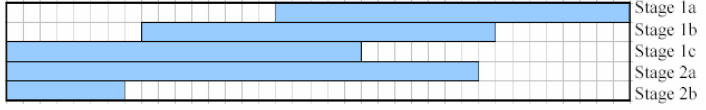
\includegraphics[width=0.45\textwidth,height=0.2\textheight,keepaspectratio]{paper_wastedarea.png}}\qquad
\subfloat[Modified Wallace Tree from~cite{betterwallace}. The image reflects the better area utilization based on the algorithm present in the paper.]{\label{fig:paper_improvedarea}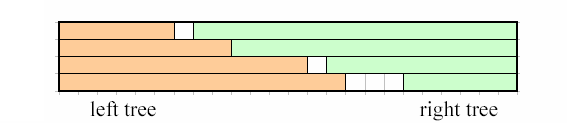
\includegraphics[width=0.45\textwidth,height=0.2\textheight,keepaspectratio]{paper_improvedarea.png}}
\caption{}
\label{fig:paper}
\end{figure}


\subsection{Implementation and Simulation Results}
\label{sec:implementation}
\subsection{Divider}


The algorithm implemented in the original version of the processor is one of the simplest but the
slowest available.

Several other algorithms can compute the division faster but all of them present disadvantages
that must be taken into account according to the target application.

Algorithms like repeated multiplication or reciprocation are fast but require a significant amount
of area, similarly an array divider would have been very fast only If we had control on the
place\&routing process in order to create a regular structure. In the end we decided to implement
a simple radix-4 division algorithm for simplicity of implementation and of the circuit itself.

Using an higher radix could have improved performance but the size of the lookup table required
by the algorithm would have increased again the area consumption.

The divider consist in a state machine (its diagram is shown in figure~\ref{fig:div_state_dia}) which checks if the inputs will
generate an overflow and performs a preliminary shift to put the divisor in the appropriate range
to be computed correctly.


\begin{figure}[H]
\centering
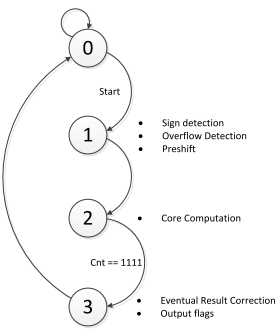
\includegraphics[width=0.85\textwidth,height=0.4\textheight,keepaspectratio]{DivisorStateMachine.png}
\caption{Divider State Diagram.}
\label{fig:div_state_dia}
\end{figure}

After that, the real computation begins and lasts 16 clock cycles. The block diagram of the divider
while it's in this state is shown in figure~\ref{fig:div_block_dia}.

\begin{figure}[H]
\centering
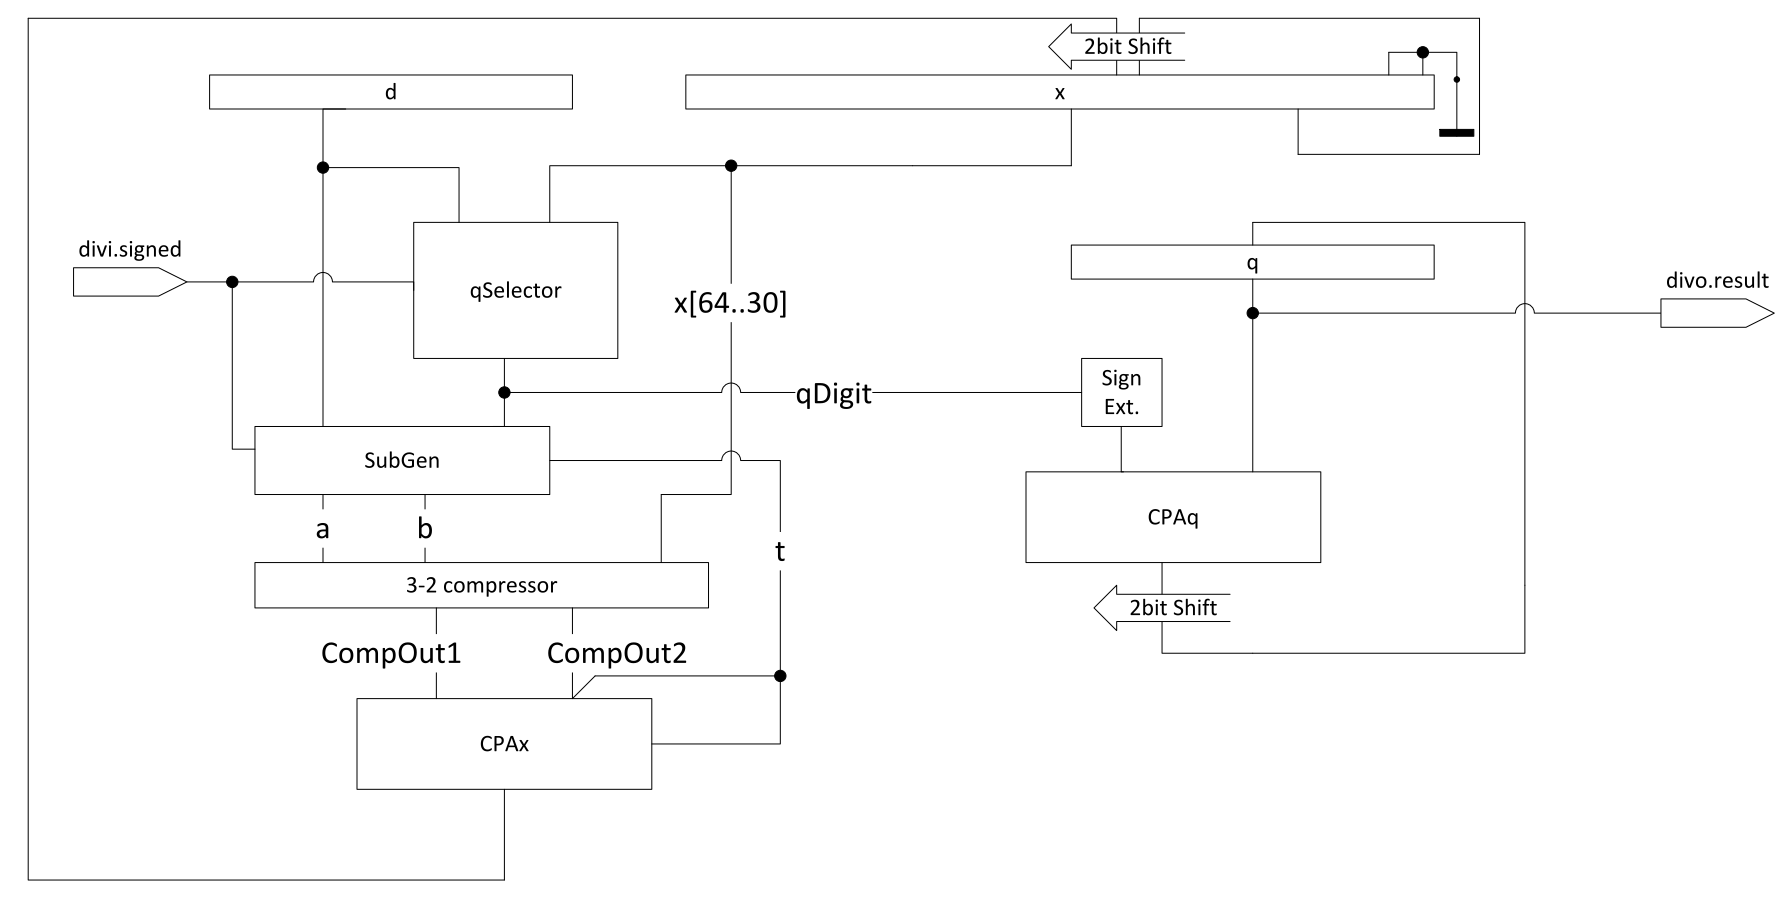
\includegraphics[width=0.85\textwidth,height=0.4\textheight,keepaspectratio]{DivisorDiagram.png}
\caption{Divider Block Diagram (during Core Computation, State = 1).}
\label{fig:div_block_dia}
\end{figure}

The algorithm is very similar to the original radix-2 version but in this case the partial reminder (x)
is shifted by 2 bits every cycle and the circuit has to guess the quotient digit from the range [-3,3].
``qSelector'' is the lookup table which performs the quotient digit guessing and it's based on the p-
d plot of the radix-4 SRT division shown in figure~\ref{fig:div_pd_plot}. In case of unsigned division only the right half of
the p-d plot is being used.

The quotient digits are in a radix-4 redundant format so a conversion to binary format is needed.
The conversion is performed gradually every cycle by the 32-bit adder ``CPAq'' which shift and sum
each generated digit with the already calculated quotient.

One could think that it would be better keep the quotient in a radix-4 redundant format and avoid
the addition in order not to slow down the execution every cycle so that the clock frequency could
be higher, but also the original divider executes a 32-bit addition every cycle so from this point of
view our divider is not worse than the original one, moreover a conversion from radix-4 redundant
format to binary is quite complicated, doing this it consists in a simple addition.

The same concept has been used also for the computation of the partial reminder.

An addition/subtraction in Carry-Save format would have been much faster and also easier, but
the selection of the quotient digit would have required the analysis of the most significant bits of
both the sum and the carry making the lookup table several orders of magnitude bigger.
In our divider ``SubGen'' generates the multiple of d to sum with the current partial reminder in a
carry save format, all this operands are been compressed by a 3-2 compressor (1 full adder of
delay) and finally the new partial reminder is calculated with a 35-bit adder, ``CPAx''

\begin{figure}[H]
\centering
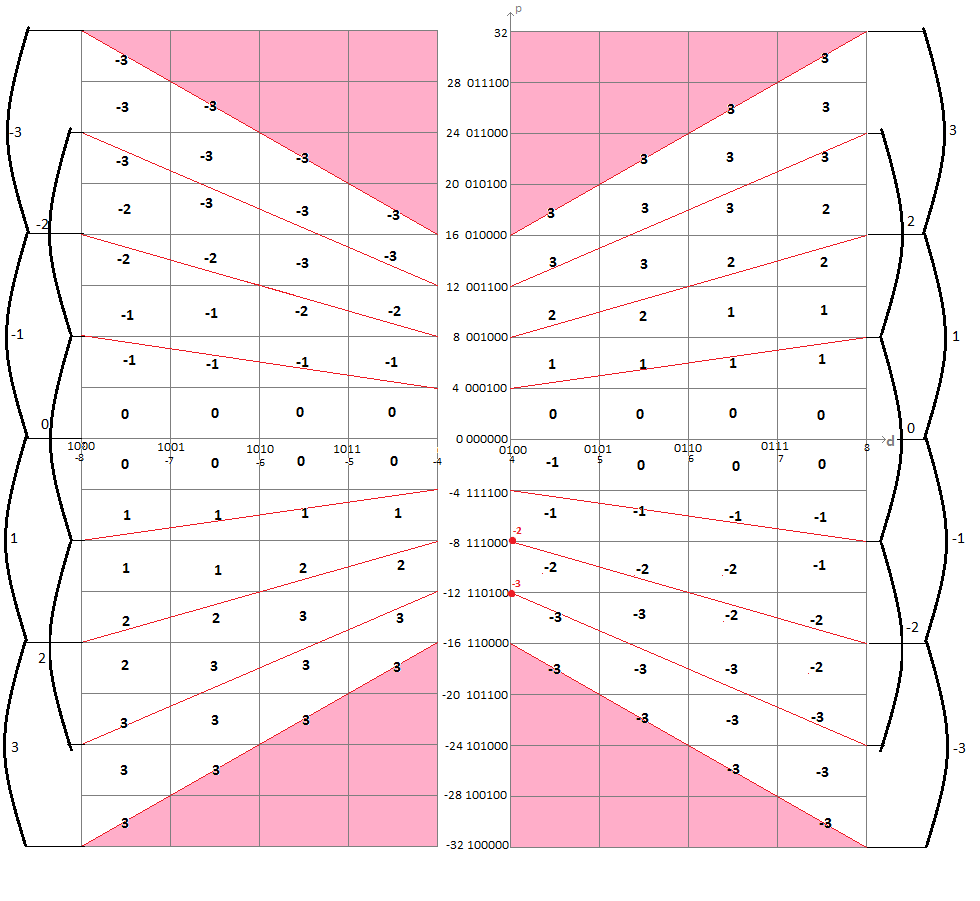
\includegraphics[width=0.85\textwidth,height=0.85\textheight,keepaspectratio]{radix4pd.png}
\caption{Radix-4 P-D Plot (Red Dots are Exceptions).}
\label{fig:div_pd_plot}
\end{figure}

Other solutions have been analyzed, such as having a lookup table only for unsigned division, half
of the size of the final version, and handle the sign separately but the synthesis has shown that the
resources utilization would have not changed significantly while one more cycle would have been needed.
Hence, we decided to keep the current divider.

At last, in order to check the compatibility of the radix-4 divider with the original one we
performed a simulation of the two versions with the same output, the only difference is in the
case of overflows where the flag is set up correctly but the result is different or in some cases
undefined, but since there is an overflow the result has no meaning so this is acceptable.

\begin{figure}[H]
\centering
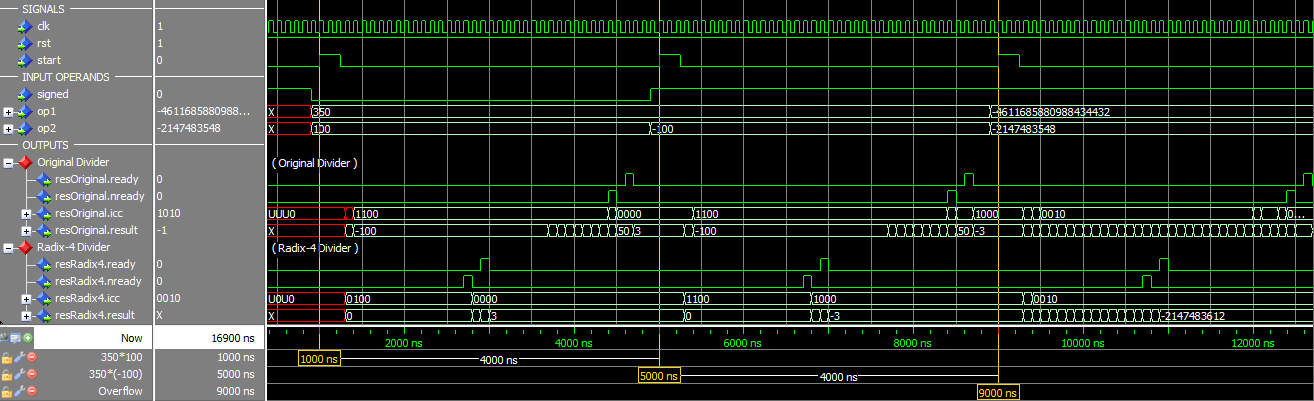
\includegraphics[width=1\textwidth,height=0.6\textheight,keepaspectratio]{myDivisionvsOriginal.png}
\caption{Signal Dump Of Radix-4 Divider Vs. Original Divider.}
\label{fig:div32_wave}
\end{figure}

\renewcommand{\kHz}{\si{\kHz}\xspace}
\renewcommand{\MHz}{\si{\MHz}\xspace}
\renewcommand{\W}{\si{\W}\xspace}
\renewcommand{\s}{\si{\s}\xspace}
\newcommand{\Oppers}{~\si[per-mode=symbol]{Op\per\s}\xspace}


\section{Results}
\label{sec:results}
\subsection{Synthesis}

In order to evaluate the performance of our improved processor we need first to play close attention to the starting point: the
performance of the baseline version of the processor.

The evaluation of each design will be divided in two main categories
\begin{itemize}
\item Resources' Utilization (provided by Xilinx ISE)
\item Benchmarks' Results (provided by the FPGA server)
\end{itemize}

The synthesis tool reported the values shown in table~\ref{tbl:resource_utilization} for the resources utilization.
Results for four different configurations are present which will allow us to better understand the impact of each modification in the area and power consumption.
These are the baseline design, the design with the modified multiplier and original divider, modified divider and original divider and finally with both units modified. 

One metric that is particularly interesting is ``P/f'' which reflects the energy efficiency of the processor. Another useful insight is the fact that the power consumption is almost proportional to the clock frequency, therefore we can use this value to estimate the power consumption at different clock frequencies.

In addition, from the synthesis report we can also see the slowest path which determines the maximum clock frequency.
This path is from \url{ddrsp0.ddrc0/ddr32.ddrc/ra.raddr_0} to \url{ddrsp0.ddrc0/ddr_phy0/ddr_phy0/xc4v.ddr_phy0/casgen}.

Those components belong to the SDRAM controller and the path is located between the controller
and the physical interface with the memory.

The cumulative synthesis report with the aforementioned four configurations is summarized in table~\ref{tbl:resource_utilization}:

\begin{table}[H]
\centering
\begin{tabular}{lcccc}
 & Baseline & Multiplier & Divider & Both\\% & Improvements\\
\midrule
Max clk freq. [\MHz] & 80.522 & 61.200 & 80.535 & 63.621\\% & \color{red} -0.39 \%\\
\# of Occupied Slices & 9904 &  11383 &  10479 & 11886\\% & \color{red} 8.77 \%\\
Total \# of 4-input LUTs & 16889 & 19589 & 17865 & 20469\\% & \color{red} 8.53 \%\\
Quiescent power [\W] & 2.467 &  2.470 & 2.468 & 2.511\\% & \color{red} 0.08 \%\\
Dynamic power [\W] & 0.721 &  0.773 & 0.743 & 0.832\\% & \color{red} 4.85 \%\\
Total power [\W] & 3.188 &  3.243 & 3.211 & 3.343\\% & \color{red} 1.16 \%\\
P/f [\si[per-mode=symbol]{\W\per\MHz}] & 0.03959 & 0.05299 & 0.03987 & 0.05255% & \color{red} 1.57 \%\\\toprule
\end{tabular}
\caption{Resource Utilization}
\label{tbl:resource_utilization}
\end{table}

The frequency is significantly hampered. This is the consequence of the low latency of the multiplier.

As expected the area consumption is higher than before as the units we designed are more complex than the baseline. In particular the lookup table in the divider, and the Wallace tree structure in the multiplier are very space-hungry. This is reflected when comparing the last and second column, with area expansion of around 18\%.

Furthermore the power consumption also augments. However the differences are more subtle, varying between 1.78\% and 15.34\%. The reason is similar, since the algorithms are more complicated more energy is expended for all the calculations. However this trade-off was envisioned at the start of the project, and as we will see later, in section~\ref{ssec:benchmarks}, the benchmark's performance improved.

Finally the power frequency ratio summarizes the points made above. Since the power consumption is higher and the frequency is lower, this metric will increase.


\subsection{Benchmark Scores}
\label{ssec:benchmarks}

Once the processor is synthesized and has been loaded in a FPGA board, Linux is initiated on the processor along with several benchmarks. In table~\ref{tbl:benchmarks} the execution times of these benchmarks are reported, for detailed scores please see the accompanying Excel file. %Unfortunately we were not able to obtain results when uploading the multiplier only design (original divider) to the FPGA. This is strange as this multiplier unit worked before, in combination with the rewritten divider. Given this evidence we suspect the problem lays with the FPGA and not with the multiplier unit.

\begin{table}[H]
\centering
\begin{tabular}{lcccc}
 & Baseline & Multiplier & Divider & Both \\
\midrule

Stanford [\s] & 2.30 & 2.25 & 2.26 & 2.31\\
Whetstone [\s] & 116.2 & 111.66 & 113.25 & 112.06\\
Gmpbench Multiply [\Oppers] & 781 & 913 & 801 & 914\\
Gmpbench Divide [\Oppers] & 15876 & 19141 & 16335 & 19205\\
Gmpbench RSA [\Oppers] & 5123 & 5342 & 5284 & 5353\\
Division [\s] & 8.06 & 7.50 & 7.65 & 7.31\\
Mibench JPEG (average) [\s] & 23.215 & 21.492 & 22.465 & 21.775\\
SSD [\s] & 10.59 & 8.70 & 10.21 & 8.60\\
Total [\s] & 219.28 & 207.98 & 203.30 & 206.92
\end{tabular}
\caption{Benchmarks Scores.}
\label{tbl:benchmarks}
\end{table}

The scores obtained with the modified processor are reported in table~\ref{tbl:benchmarks}. As one can see introducing the divider has a widespread positive effect on the scores. The same can be said about the multiplier. Analyzing these results with respect to the worst area and power performance will be left for section~\ref{ssec:metrics}.

From these results we can see that almost every benchmark had a healthy improvement, in the end
the total execution time improved by 5.64\%.
It is interesting to observe that both units yield improvements to the benchmark scores.
% However for the total execution time introducing the multiplier has a detrimental effect.
% This is counter-intuitive given there were improvements in all the individual benchmark scores.
% \textcolor{red}{\large The reason for this behavior is not clear to us.}

These scores are not as good as expected but likely the execution of the operating system
on the processor causes a non negligible overhead in the execution due to the scheduling. As an example, the
divider takes about half the time to execute but the execution time of the division related
benchmarks is only about 10\% better.

\subsection{Metrics Comparison}
\label{ssec:metrics}

In order to get a fair comparison between the baseline and the improved processor some standard
metrics have to be calculated and studied.

Usually these metrics are \texttt{A}, the area consumption here calculated as the weighted sum of the
number of occupied slices and the number of 4-input LUTs used where the weight is the reciprocal
of the number of available resources, \texttt{D} is the delay or the reciprocal of the maximum clock frequency
and indicate the delay of the slowest path, \texttt{P} is the power and it's simply calculated as the total
power consumed by the Dhrystone benchmark used for the simulation and \texttt{BS} is the benchmark
score which indicate how fast a program can be executed, it's calculated as the total execution
time of the benchmarks on the FPGA board.

For the area we are using the weighted formula to account for the true cost of our implementation instead of just the number of resources used.
We make the simplistic assumption that the number of resources available on the device is inversely proportional to their effective cost. Thus we use their reciprocal as a weight to calculate the average. Therefore we obtain a metric which is likely similar to the actual cost of the implementation on a chip.

Moreover some composite metrics can be observed. These metrics consider two or more primitive
metrics and are often more interesting than the latter because improvements in one metric are usually accompanied by decrease in other.
Thus composite metrics show the overall performance, and give insight on the necessary trade-offs.

Since we want to speed-up the execution of the software while keeping the power consumption
low as our target applications are embedded systems, the composite metric we are
interested the most is \texttt{P$\times$BS}. It reflects how much the processor is able to compute for the same unit of energy.

Additional composite metrics are \texttt{A$\times$D}, \texttt{A$\times$BS} and \texttt{P$\times$D}. Since we focused on the
execution time and power consumption one can notice that the other metrics are worse in our version
compared to the baseline.

All the baseline's and modified units' synthesis and benchmark results have been condensed in table~\ref{tbl:final_metrics}.

\begin{table}[H]
\centering

\resizebox{\textwidth}{!}{ %scales the font automagically to fit the maximum text width! Nice :)
\begin{tabular}{lcccc}
&
\multicolumn{4}{c}{Primitive Metrics}\\
&
\ttfamily A &
\ttfamily D &
\ttfamily P &
\ttfamily BS \\
Baseline &
\num{2.68E+04} &
\num{1.24E-02} &
\num{3.19E+00} &
\num{2.19E+02} \\
Modified (Mul)&
\num{3.10E+04} &
\num{1.63E-02} &
\num{3.24E+00} &
\num{2.07E+02} \\
Modified (Div)&
\num{2.83E+04} &
\num{1.24E-02} &
\num{3.21E+00} &
\num{2.03E+02} \\
Modified (Mul\&Div)&
\num{3.24E+04} &
\num{1.57E-02} &
\num{3.34E+00} &
\num{2.07E+02} \\
Improvements (Mul) &
\color{red} 			15.6\% &
\color{red} 			31.5\% &
\color{red} 			1.6\% &
\color{green!60!black} 	-5.0\% \\
Improvements (Div) &
\color{red} 5.8\% &
\color{orange} 0.0\% &
\color{red} 0.7\% &
\color{green!60!black} -7.3\% \\
Improvements (Mul\&Div) &
\color{red} 21.0\% &
\color{red} 41.1\% &
\color{red} 5.0\% &
\color{green!60!black} -6.0\% \\

\\ \midrule \\

& \multicolumn{4}{c}{Composite Metrics}\\
&
\ttfamily A$\times$D &
\ttfamily A$\times$BS &
\ttfamily P$\times$D &
\ttfamily P$\times$BS\\
Baseline &
\num{3.33E+02} &
\num{5.88E+06} &
\num{3.96E-02} &
\num{6.99E+02} \\
Modified (Mul)&
\num{5.05E+02} &
\num{6.42E+06} &
\num{5.28E-02} &
\num{6.71E+02} \\
Modified (Div)&
\num{3.52E+02} &
\num{5.75E+06} &
\num{3.99E-02} &
\num{6.52E+02} \\
Modified (Mul\&Div)&
\num{5.09E+02} &
\num{6.69E+06} &
\num{5.24E-02} &
\num{6.92E+02} \\
Improvements (Mul) &
\color{red} 			51.7\% &
\color{red} 			9.2\% &
\color{red} 			33.3\% &
\color{green!60!black} 	-4.0\% \\
Improvements (Div) &
\color{red} 5.8\% &
\color{green!60!black} -2.2\% &
\color{red} 0.7\% &
\color{green!60!black} -6.7\% \\
Improvements (Mul\&Div)&
\color{red} 52.9\% &
\color{red} 2.6\% &
\color{red} 32.32\% &
\color{green!60!black} -1.1\%\\
\end{tabular}}
\caption{Final Metrics For Baseline And Improved Versions.}
\label{tbl:final_metrics}
\end{table}

Interpreting the table is very straightforward: the modifications introduced a penalty on the area and power but delivered better benchmark performance. This is not as surprising result as this trade off had been identified and explained at the beginning of this document. In particular the multiplier has an important impact on the delay and the power consumption. Future work would necessarily include improvements in this aspects.

As stated in the introduction our main target was to decrease the computation time while keeping the power consumption as low as possible, which is reflected in the \texttt{P $\times$ BS}. Given we have a 1.1\% improvement in that metric we can conclude our main goal was accomplished. Unfortunately the results were not as impressive as desired but, as mentioned previously, this maybe due to scheduling overhead.

It would be interesting to analyze in detail the benchmarks as future work in order to better understand how improvements in the arithmetic units impact them. Alternatively using handpicked subsets of these benchmarks to obtain a more fine-grained picture of their execution could be beneficial to this study. After obtaining significant insight from this work it would be possible to iteratively modify the arithmetic units (among others) to yield better benchmark results at a lower power consumption and circuit footprint.
Moreover a thorough inspection of the processor could also identify other areas for improvement, some of those were mentioned in this report. 

\section{Conclusions and further improvements}

The improvements made to the arithmetic units have improved the benchmark performance of the processor. Although they are modest, they reflect the chosen target scenario.

Because of lack of time we were unable to perform more changes, but of course there are many things to
change in the architecture to improve further the performance.

Different configurations for the multiplier should have been tested to decrease its impact on power and maximum frequency.

The size and structure of the cache memory could be changed to decrease the probability of misses and consequently the benchmarks execution time. Although this could have been done using the configuration tool it
would have not been fruit of our own merit. Moreover increasing the cache size probably would
have increased also the power consumption, escalating even more this issue.

The LEON3 uses a static branch prediction in the integer unit, which is a good compromise
between power consumption, as no difficult computation is needed, yet there are gains in terms of execution time.
To improve performance further, a 1 bit or a 2 bit branch prediction buffer
algorithm could be implemented. The calculations needed are more intricate and computed more often (30\% of
the instructions are branches) henceforth the power consumption would probably increase. On the other hand the gains in terms of execution time could make up for the loss.

In the end another heavy modification that could have been done is making the
integer unit super-scalar and implementing Out of Order execution. Hypothetically it could yield 
significant performance improvements in terms of execution time. Notwithstanding a complete re-design of the integer unit
would have been needed, which deemed it impossible to complete in the (small) time budget for this project.
%referências

\phantomsection
\begin{thebibliography}{15}

\bibitem{book}
CA book

\bibitem{betterwallace}
betterwallace

\bibitem{doc}
doc

\bibitem{part3}
part3


\end{thebibliography}

%\phantomsection
\appendix

\section{Baseline}
\subsection{Dhrystone report}
\label{app:A}


\section{Improved Version}
\subsection{Dhrystone report}



\end{document}
